\documentclass[a4paper,12pt]{article}

% --- Шрифты и кодировки ---
\usepackage[utf8]{inputenc}
\usepackage[T1]{fontenc}
\usepackage[russian]{babel}
\usepackage{mathptmx} % Times New Roman

% --- Поля ---
\usepackage[left=3cm, right=1.5cm, top=2cm, bottom=2cm]{geometry}

% --- Межстрочный интервал ---
\usepackage{setspace}
\onehalfspacing % Интервал 1.5

% --- Абзацы ---
\setlength{\parindent}{1.25cm} % Красная строка
\setlength{\parskip}{0pt}      % Без межабзацного отступа

% --- Графика и вёрстка ---
\usepackage{graphicx}
\usepackage{pgfplots}
\pgfplotsset{compat=1.18}
\usepackage{svg}
\usepackage{float}
\usepackage{qrcode}

% --- Математика ---
\usepackage{amsmath}

% --- Программный код ---
\usepackage{minted}
% \usepackage{listings}
% \lstset{
%     language=Python,
%     basicstyle=\ttfamily\small,
%     numbers=left,
%     numberstyle=\tiny,
%     stepnumber=1,
%     numbersep=5pt,
%     frame=single,
%     breaklines=true,
%     showstringspaces=false,
%     tabsize=4
% }

% --- Прочее ---
\usepackage{titling}
\usepackage{enumitem}
\usepackage{tocloft}
\renewcommand{\cftsecleader}{\cftdotfill{\cftdotsep}}

% --- Гиперссылки ---
\usepackage[hidelinks]{hyperref}

\begin{document}

\tableofcontents
\newpage

\section{Введение} 
Вращательное движение часто встречается как в природе, так и в инженерных системах: от движения воздушных масс в атмосфере до вращающихся механизмов в технике. При анализе движения тел в таких системах необходимо учитывать дополнительные силы, возникающие вследствие вращения системы отсчёта. Одной из таких инерциальных сил является сила Кориолиса.

Сила Кориолиса представляет собой фиктивную силу, возникающую при рассмотрении движения тела в неинерциальной вращающейся системе отсчёта. Её учет имеет важное значение при моделировании широкого круга физических процессов, таких как динамика атмосферы и океанов, движение снарядов, гироскопические эффекты и другие явления, связанные с вращением.

Целью данной работы является исследование особенностей движения тела на вращающемся диске с учётом действия силы Кориолиса, а также построение математической модели такого движения. В процессе работы будет проведён анализ уравнений движения, численное моделирование и интерпретация полученных результатов.

\newpage
\section{Формализация}

\subsection{Тело (материальная точка)}

\textbf{Обозначение:} $\vec{r}(t) = (x(t), y(t))$ — положение тела на вращающемся диске в момент времени $t$. \\
Характеристики:
\begin{itemize}
    \item \textbf{Масса:} Обозначается как $m$. Используется при вычислении силы Кориолиса.
    \item \textbf{Начальные условия:} Начальное положение и скорость: $\vec{r}_0 = (x_0, y_0)$, $\vec{v}_0 = (\dot{x}_0, \dot{y}_0)$.
    \item \textbf{Скорость и ускорение:} Производные от координат по времени: $\vec{v}(t) = \dot{\vec{r}}(t)$, $\vec{a}(t) = \ddot{\vec{r}}(t)$.
\end{itemize}
Допущения:
\begin{itemize}
    \item Тело моделируется как материальная точка — размер и форма не учитываются.
    \item Действие сопротивления среды (воздуха, трения и т.п.) не рассматривается.
    \item Масса тела постоянна во времени.
\end{itemize}

\subsection{Вращающийся диск}

\textbf{Обозначение:} $\vec{\omega} = (0, 0, \omega)$ — вектор угловой скорости вращения диска вокруг оси $z$. \\
Характеристики:
\begin{itemize}
    \item \textbf{Плоскость движения:} Движение происходит в горизонтальной плоскости $XY$.
    \item \textbf{Радиус диска:} Обозначается как $R$; движение рассматривается только внутри области $|\vec{r}(t)| \leq R$.
    \item \textbf{Угловая скорость:} $\omega = \text{const}$ — постоянная величина.
\end{itemize}
Допущения:
\begin{itemize}
    \item Диск вращается равномерно (без ускорения).
    \item Диск считается абсолютно жёстким и несжимаемым.
    \item Колебания, деформации и трение в подложке не учитываются.
\end{itemize}

\textbf{Допущения по силам:}
\begin{itemize}
    \item Гравитация и сопротивление воздуха отсутствуют или несущественны.
    \item Моделируется только сила Кориолиса. Центробежная сила не учитывается.
    \item Моделирование ведётся в системе отсчёта, связанной с вращающимся диском.
\end{itemize}

\newpage

\section{Составление математической модели}

Для описания движения тела удобно использовать декартову систему координат $(x, y)$ в плоскости диска, вращающегося вокруг оси $z$ с постоянной угловой скоростью $\omega$. Радиус-вектор положения тела:
\[
\vec{r}(t) = x(t)\hat{i} + y(t)\hat{j}
\]
Скорость тела:
\[
\vec{v}(t) = \frac{d\vec{r}}{dt} = \dot{x}(t)\hat{i} + \dot{y}(t)\hat{j}
\]
Угловая скорость вращения диска:
\[
\vec{\omega} = (0, 0, \omega)
\]

\subsection{Общий вид уравнения движения в неинерциальной системе}

%% ИЗМЕНЕНИЕ: Уравнение упрощено, убран член центробежной силы.
Во вращающейся системе отсчёта, если учитывать только силу Кориолиса, второй закон Ньютона принимает вид:
\[
m \vec{a}' = \vec{F}_\text{реальные} - 2m (\vec{\omega} \times \vec{v}')
\]
где:
\begin{itemize}
    \item $\vec{a}'$ — ускорение в системе, связанной с диском;
    \item $\vec{F}_\text{реальные}$ — реальные силы (в данной модели отсутствуют, $\vec{F}_\text{реальные} = 0$);
    \item $-2m (\vec{\omega} \times \vec{v}')$ — сила Кориолиса.
\end{itemize}
Сократив массу $m$, получаем уравнение для ускорения:
\[
\vec{a}' = -2 (\vec{\omega} \times \vec{v}')
\]

\subsection{Вычисление силы Кориолиса в декартовых координатах}

%% ИЗМЕНЕНИЕ: Убрано вычисление для центробежной силы.
Векторное произведение для силы Кориолиса:
\[
\vec{\omega} \times \vec{v} =
\begin{pmatrix}
0 \\ 0 \\ \omega
\end{pmatrix}
\times
\begin{pmatrix}
\dot{x} \\ \dot{y} \\ 0
\end{pmatrix}
=
\begin{pmatrix}
-\omega \dot{y} \\
\omega \dot{x} \\
0
\end{pmatrix}
\]
Тогда ускорение Кориолиса равно:
\[
\vec{a}' = -2(\vec{\omega} \times \vec{v}) =
\begin{pmatrix}
2\omega \dot{y} \\
-2\omega \dot{x} \\
0
\end{pmatrix}
\]

\subsection{Итоговая система дифференциальных уравнений}

%% ИЗМЕНЕНИЕ: Уравнения теперь содержат только компоненты ускорения Кориолиса.
Подставим компоненты ускорения в уравнение движения, спроецировав его на оси $x$ и $y$:
\[
\ddot{x}(t) = 2\omega \dot{y}(t)
\]
\[
\ddot{y}(t) = -2\omega \dot{x}(t)
\]
Эта система описывает траекторию тела под действием исключительно силы Кориолиса.

\newpage

\section{Численные эксперименты}

Для анализа поведения тела на вращающемся диске были проведены численные эксперименты. Основная цель — исследовать, как начальные условия и угловая скорость диска влияют на траекторию движения, когда действует только сила Кориолиса. Для решения системы уравнений использован метод Эйлера.

\subsection*{Выбор параметров модели}

Во всех экспериментах используются одинаковые параметры модели:
\begin{itemize}
    \item $R = 5.0$ — радиус вращающегося диска;
    \item $dt = 0.01$ — шаг по времени;
    \item $T = 20.0$ — общая длительность эксперимента.
\end{itemize}

\newpage

%% ИЗМЕНЕНИЕ: Описания экспериментов и пути к файлам обновлены.

\subsection*{Эксперимент 1: $\omega = 1.0$, $(x_0, y_0) = (1.0, 0.0)$, $(v_{x0}, v_{y0}) = (0.0, 2.0)$}
\begin{itemize}
    \item Сила Кориолиса, действуя перпендикулярно скорости, заставляет тело двигаться по окружности.
    \item Траектория представляет собой идеальную окружность, так как отсутствуют другие силы.
\end{itemize}
\begin{figure}[H]
    \centering
    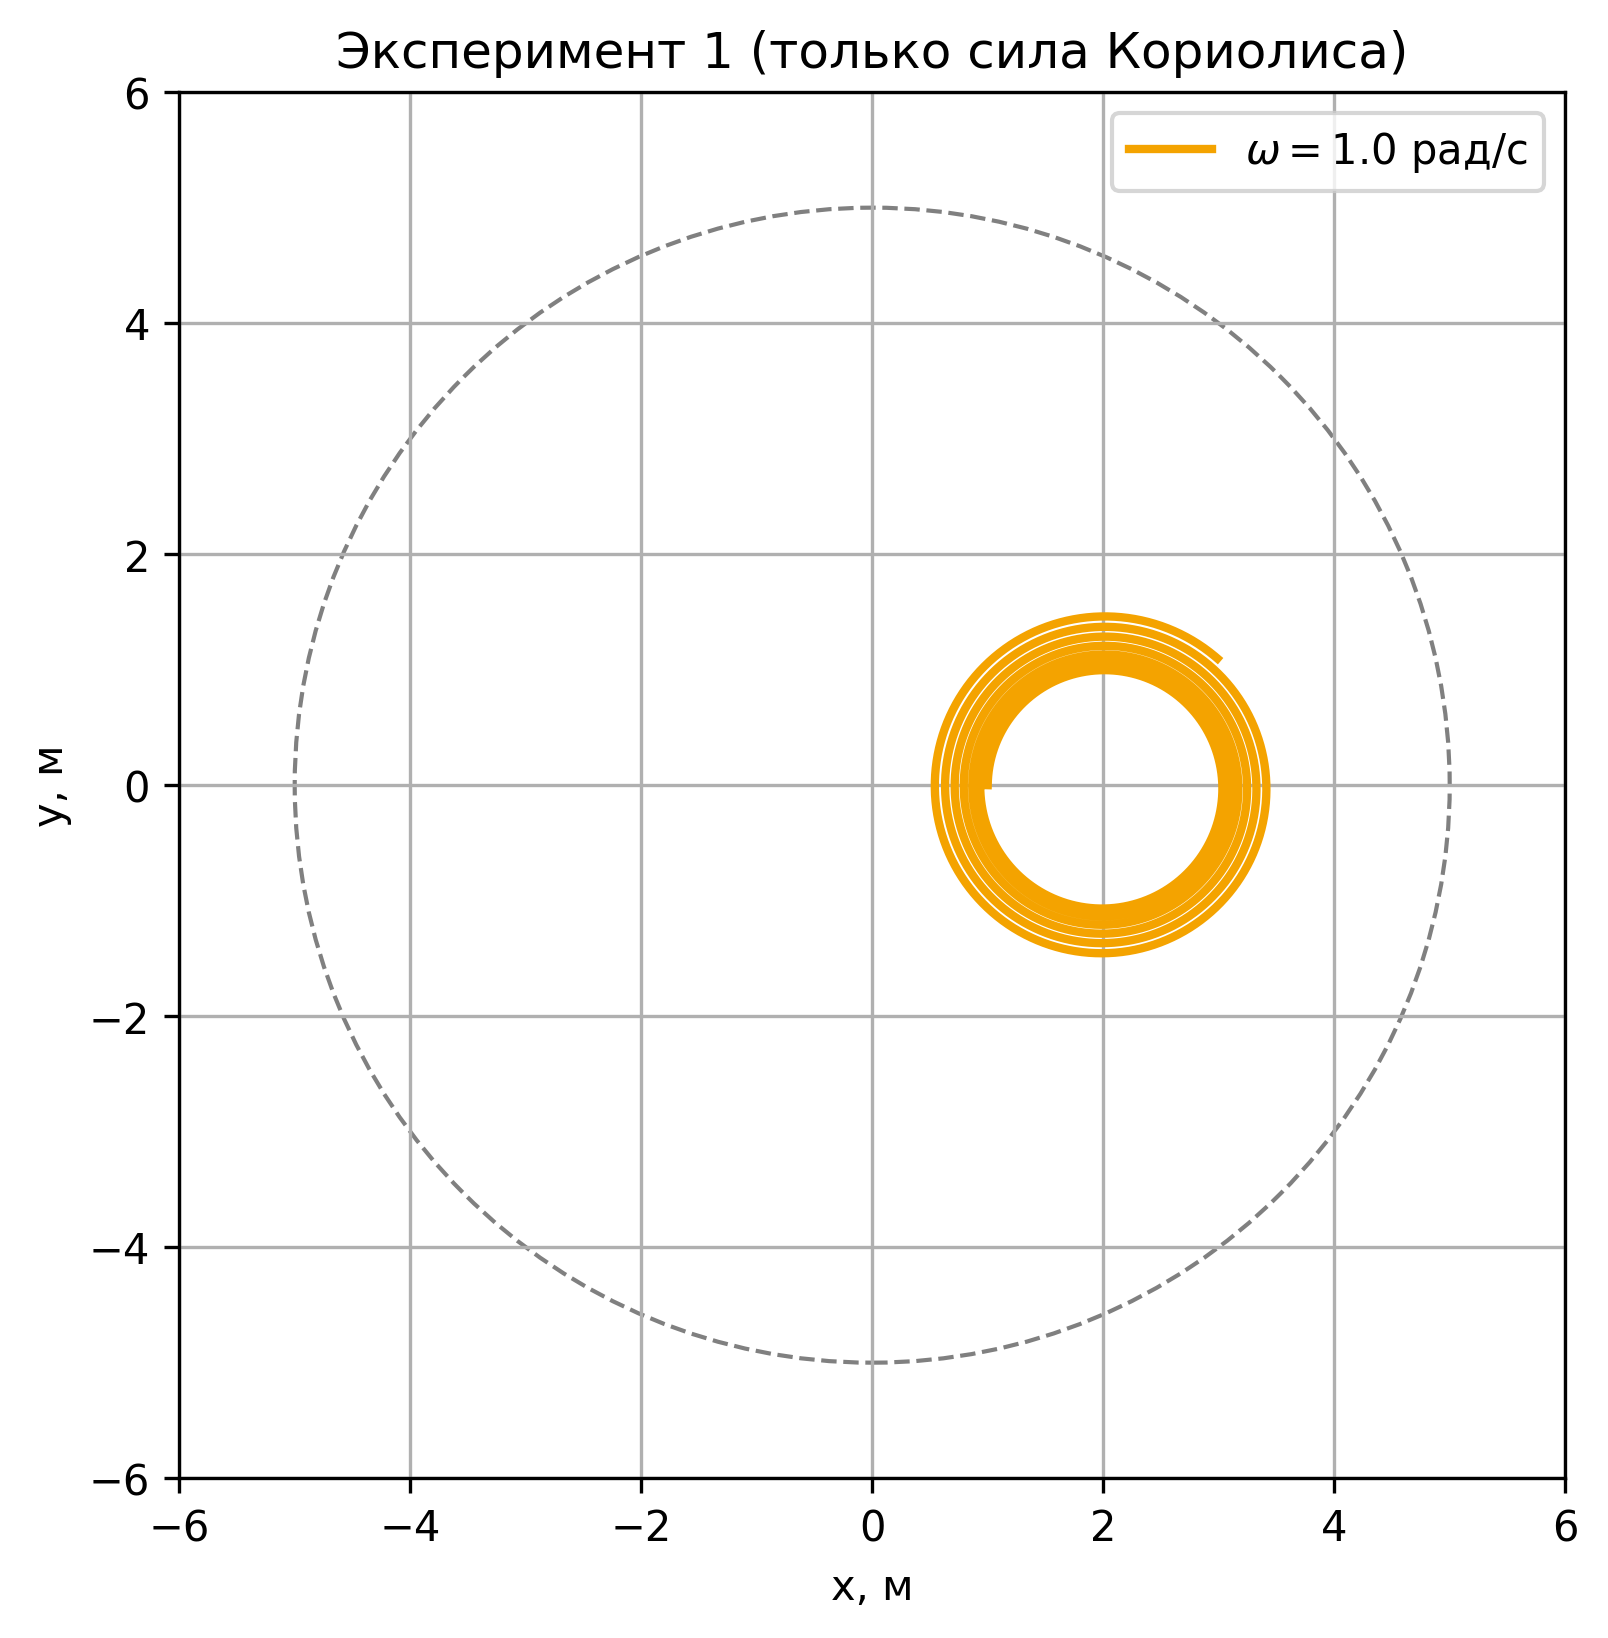
\includegraphics[width=0.8\textwidth]{plots_coriolis_only/experiment_1.png}
    \caption{Траектория движения тела (Эксперимент 1)}
\end{figure}

\newpage

\subsection*{Эксперимент 2: $\omega = 2.0$, $(x_0, y_0) = (0.0, 1.0)$, $(v_{x0}, v_{y0}) = (2.0, 0.0)$}
\begin{itemize}
    \item Увеличение угловой скорости $\omega$ приводит к увеличению силы Кориолиса.
    \item В результате радиус окружности, по которой движется тело, уменьшается.
\end{itemize}
\begin{figure}[H]
    \centering
    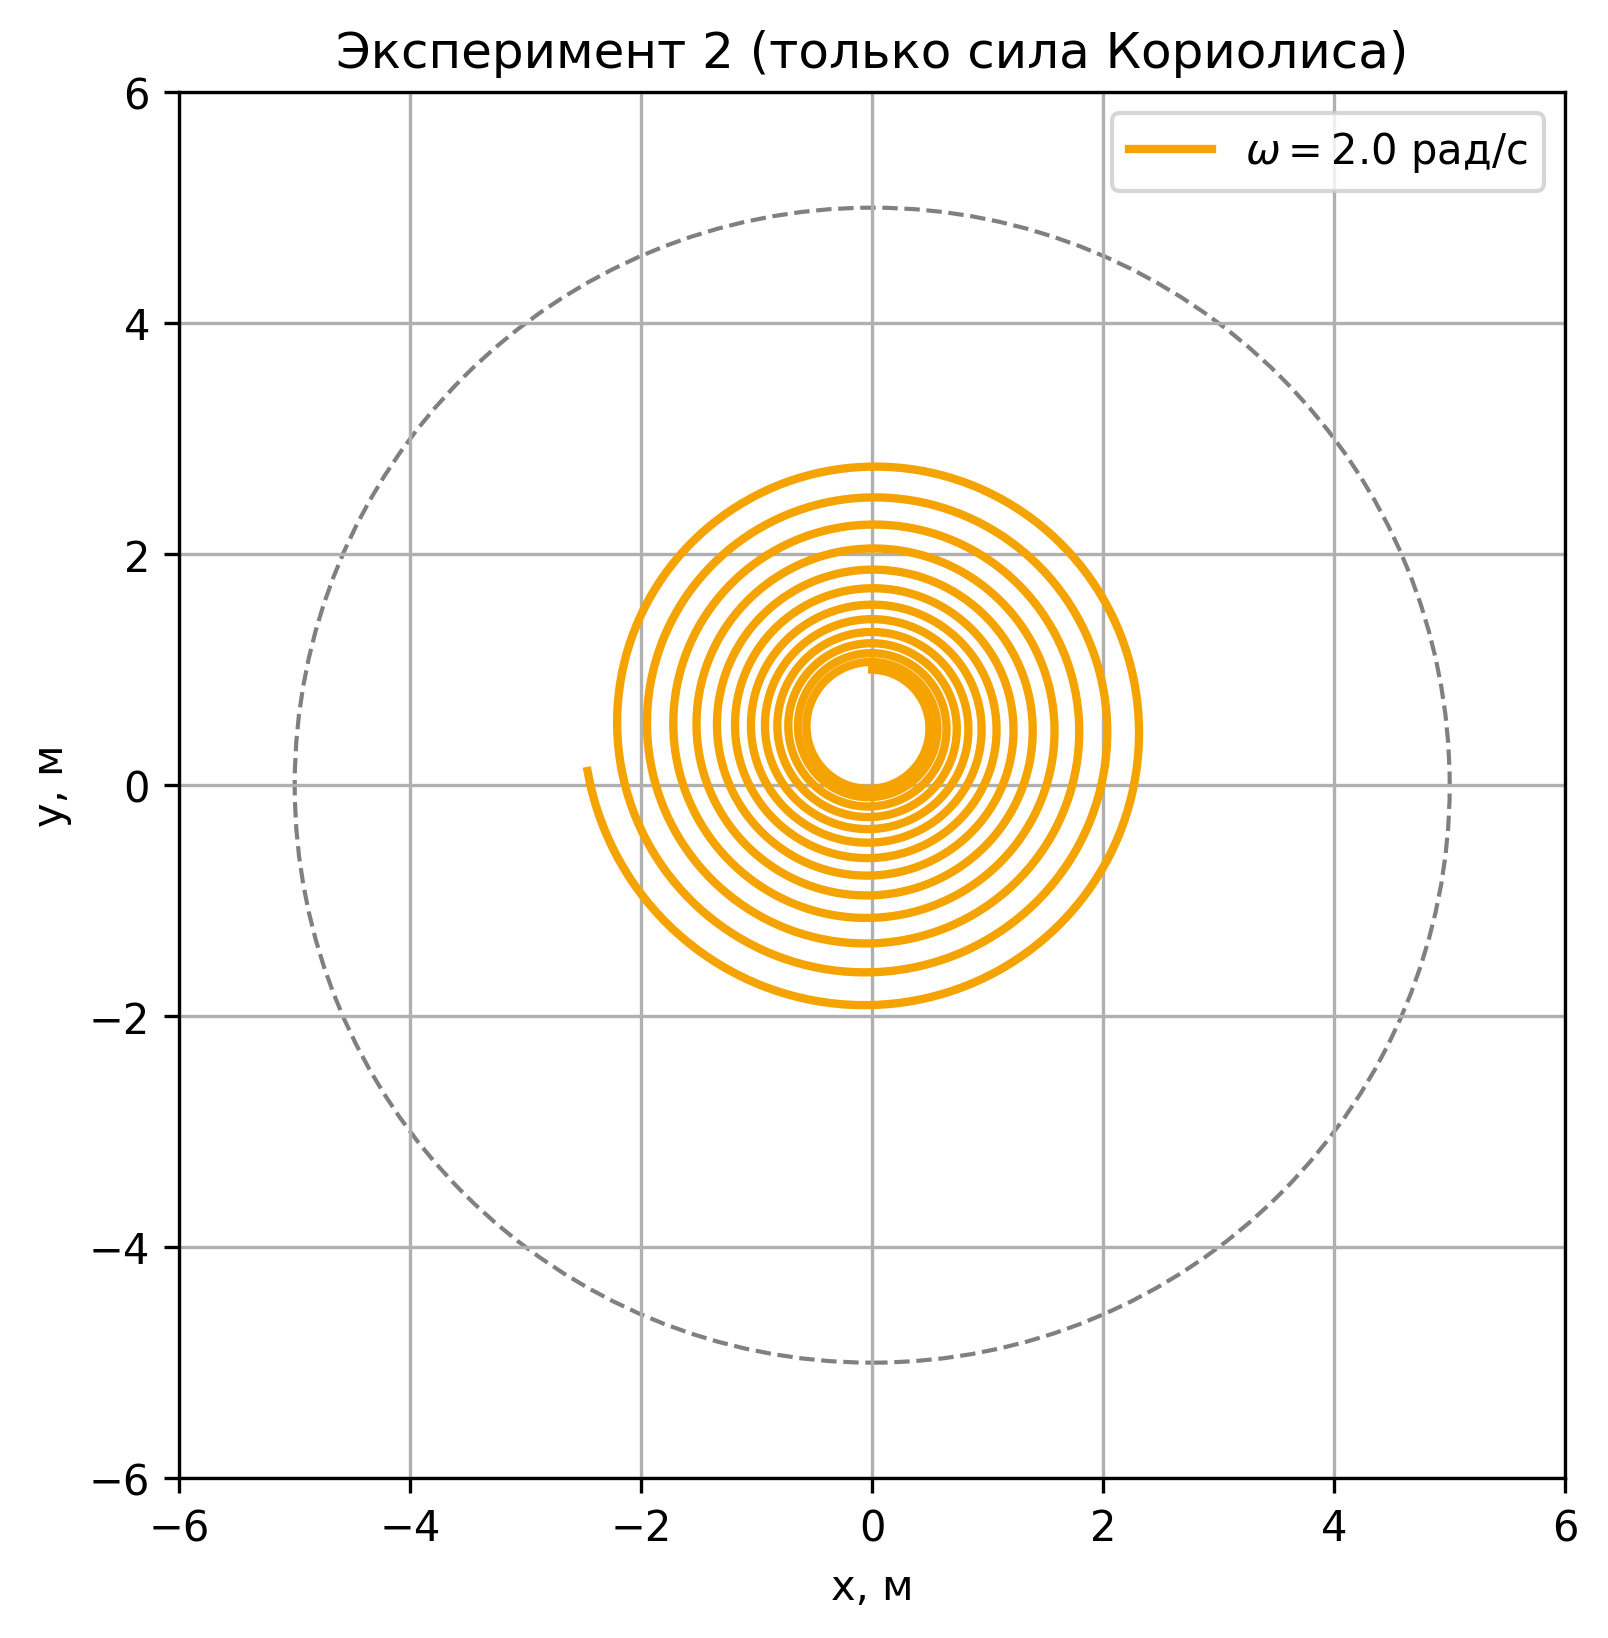
\includegraphics[width=0.8\textwidth]{plots_coriolis_only/experiment_2.png}
    \caption{Траектория движения тела (Эксперимент 2)}
\end{figure}

\newpage

\subsection*{Эксперимент 3: $\omega = 3.0$, $(x_0, y_0) = (2.0, 0.0)$, $(v_{x0}, v_{y0}) = (0.0, 1.5)$}
\begin{itemize}
    \item При высокой угловой скорости $\omega$ радиус траектории становится еще меньше.
    \item Тело совершает движение по окружности малого радиуса вблизи точки старта.
\end{itemize}
\begin{figure}[H]
    \centering
    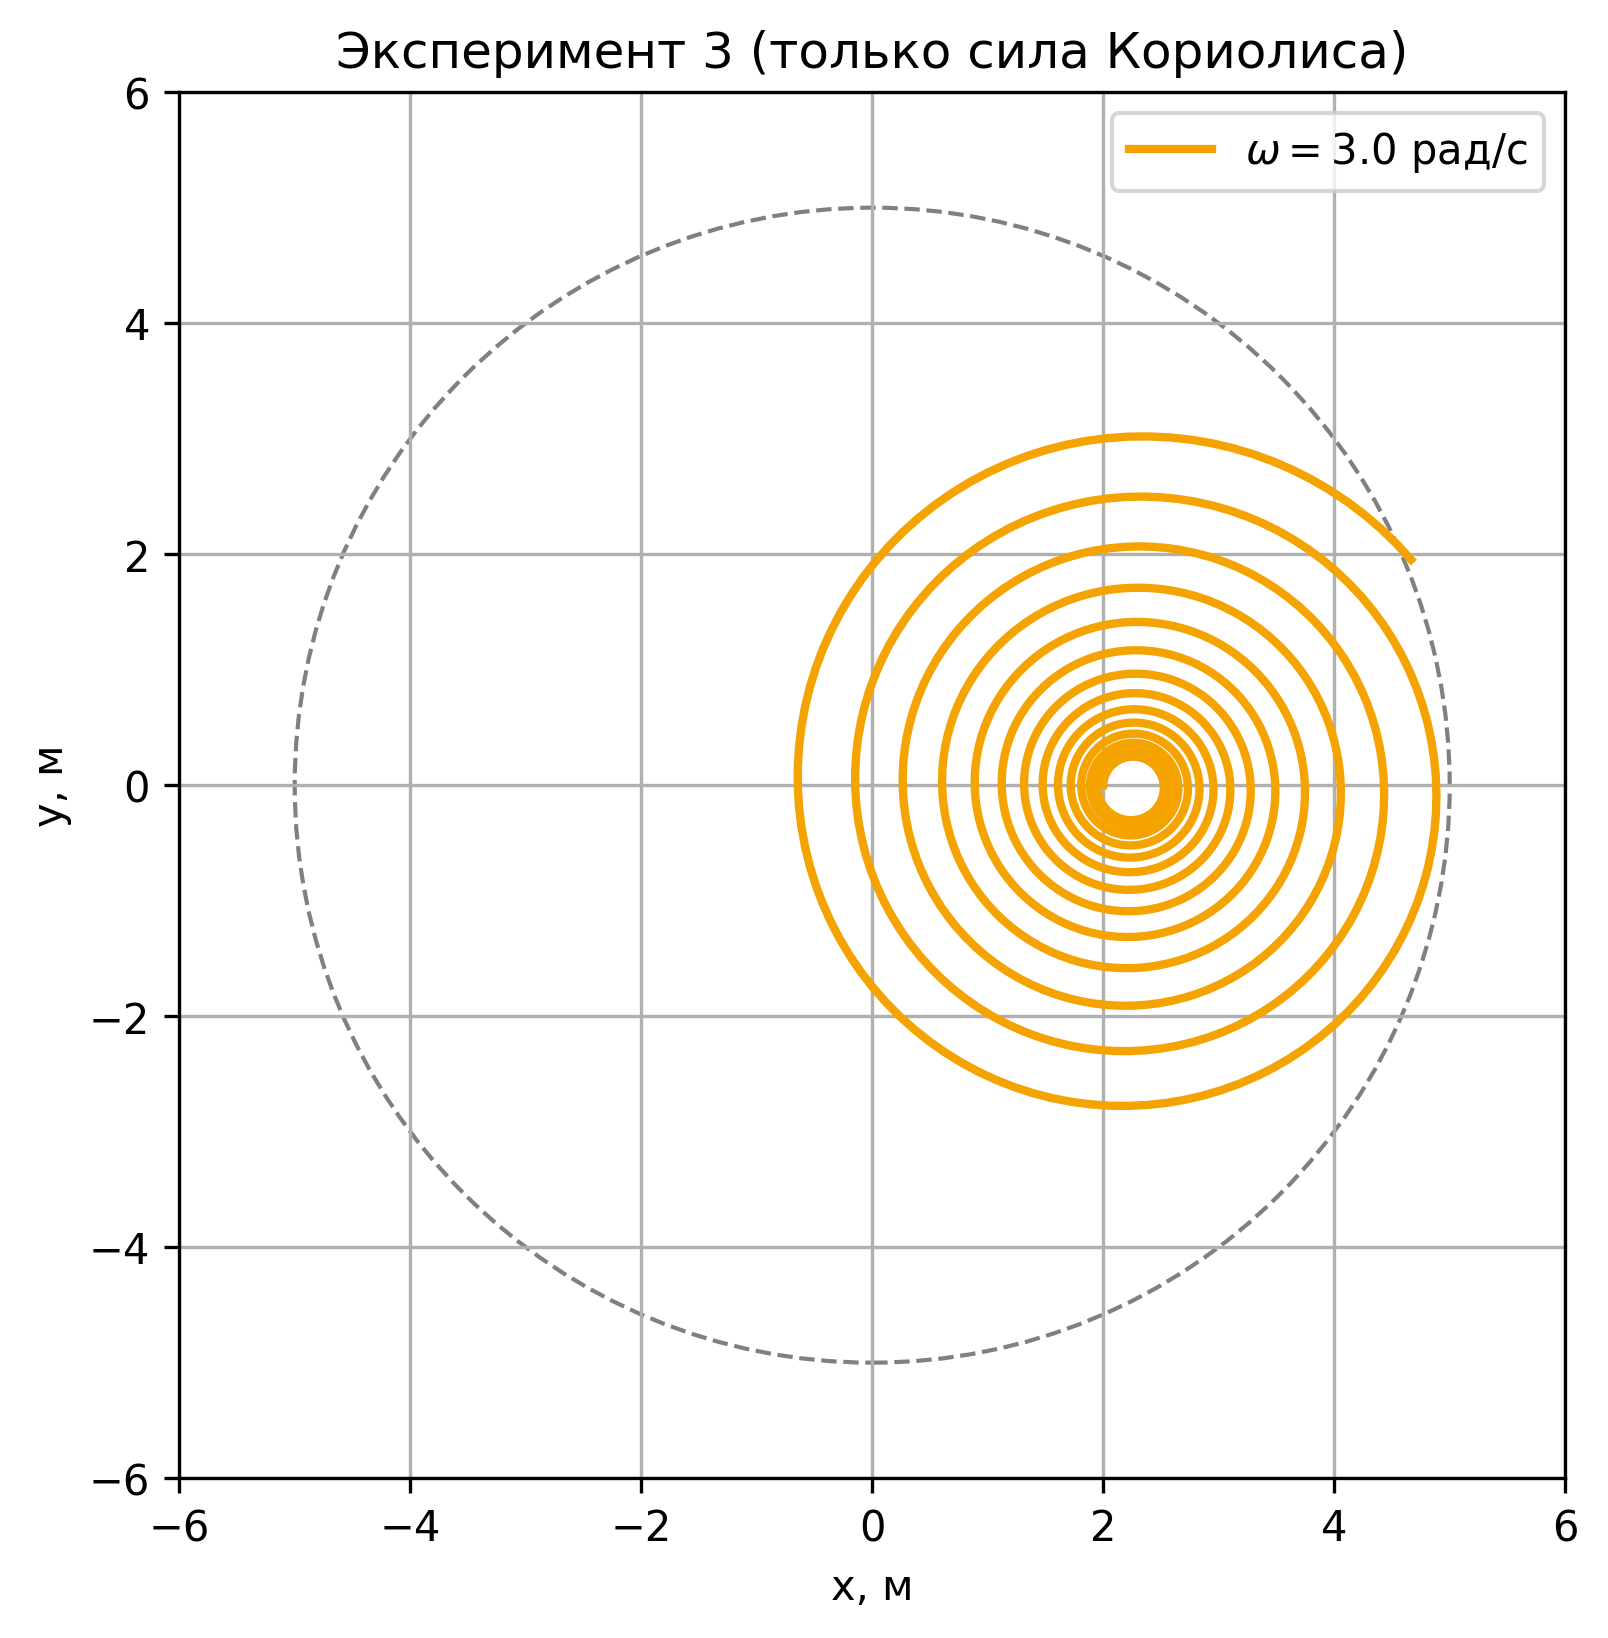
\includegraphics[width=0.8\textwidth]{plots_coriolis_only/experiment_3.png}
    \caption{Траектория движения тела (Эксперимент 3)}
\end{figure}

\newpage

\subsection*{Эксперимент 4: $\omega = 1.5$, $(x_0, y_0) = (1.0, 1.0)$, $(v_{x0}, v_{y0}) = (1.0, -1.0)$}
\begin{itemize}
    \item Независимо от направления начальной скорости, траектория всегда является окружностью.
    \item Сила Кориолиса постоянно отклоняет вектор скорости, формируя замкнутый круговой путь.
\end{itemize}
\begin{figure}[H]
    \centering
    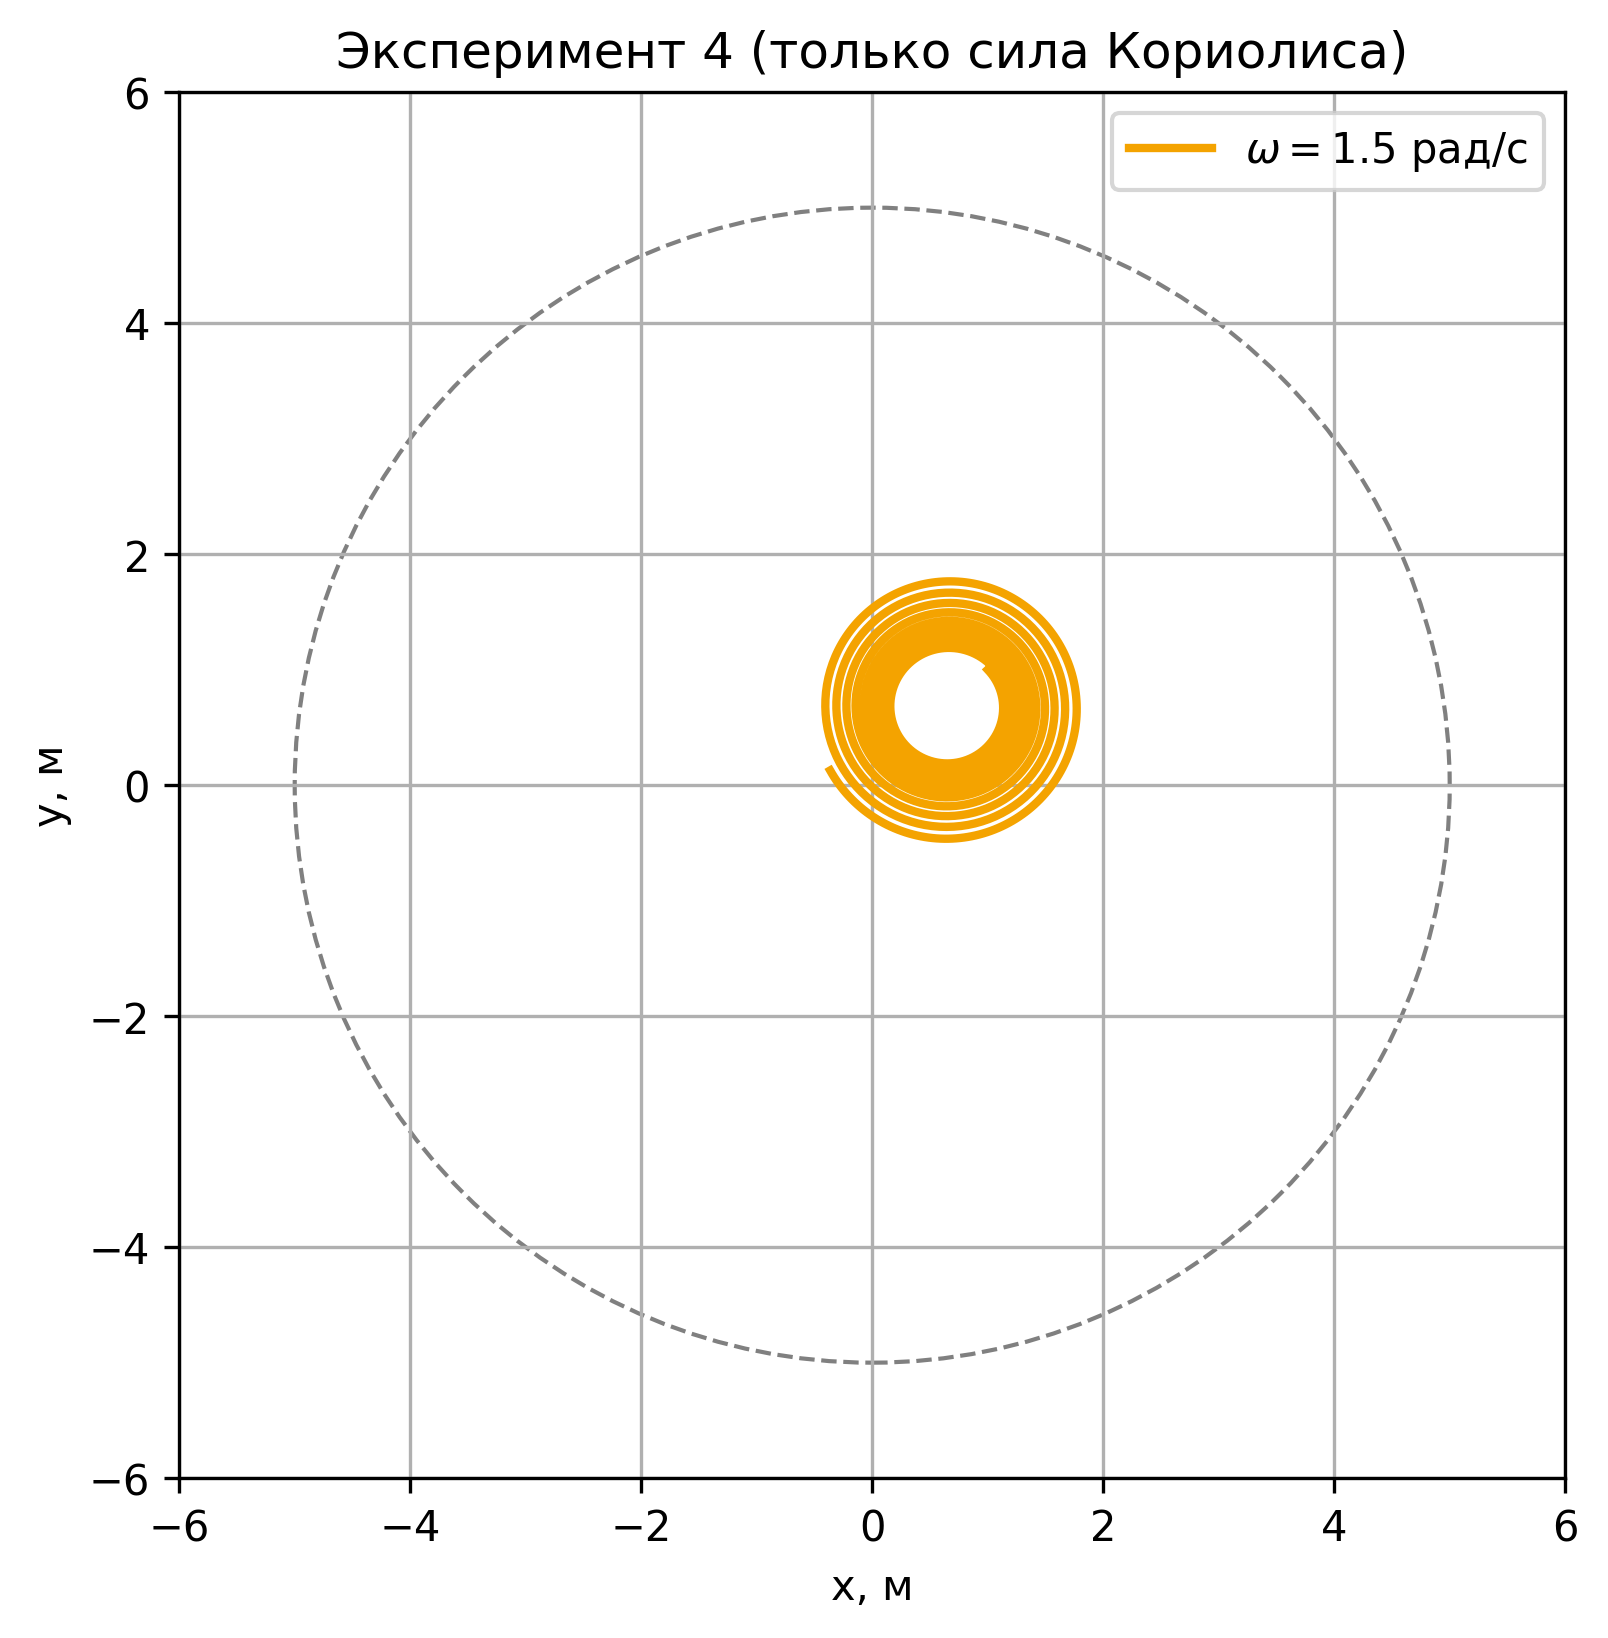
\includegraphics[width=0.8\textwidth]{plots_coriolis_only/experiment_4.png}
    \caption{Траектория движения тела (Эксперимент 4)}
\end{figure}

\newpage

\subsection*{Анализ результатов численных экспериментов}
Во всех экспериментах отчётливо проявляется влияние силы Кориолиса на траекторию тела:
\begin{itemize}
    \item Траектория движения во всех случаях является окружностью, что соответствует теории.
    \item Радиус этой окружности обратно пропорционален угловой скорости $\omega$: чем больше $\omega$, тем меньше радиус кругового движения.
    \item Начальные условия (положение и скорость) определяют центр и радиус этой окружности.
    \item Модель эффективно демонстрирует "чистое" действие силы Кориолиса.
\end{itemize}
Таким образом, численные эксперименты подтверждают корректность модели для случая с единственной силой Кориолиса.

\newpage

\section{Выводы}

В ходе выполнения работы была построена и исследована математическая модель движения тела под действием только силы Кориолиса. Для численного решения уравнений использовался метод Эйлера.

На основе проведённых экспериментов можно сделать следующие выводы:
\begin{itemize}
\item \textbf{Характер траекторий}: При наличии только силы Кориолиса траектория движения тела всегда является окружностью. Ее радиус зависит от начальной скорости тела и угловой скорости вращения системы.
\item \textbf{Сила Кориолиса}: Модель адекватно описывает влияние этой силы. Будучи всегда перпендикулярной вектору скорости, она не совершает работы и не меняет модуль скорости, а лишь изменяет ее направление, что и приводит к движению по окружности.
\item \textbf{Физический смысл модели} подтверждён визуализацией: траектории согласуются с ожидаемым поведением (инерционные круги).
\item \textbf{Численный метод} продемонстрировал устойчивость и достаточную точность для визуального анализа при выбранных параметрах.
\end{itemize}

Таким образом, численное моделирование позволило наглядно продемонстрировать эффект "чистой" силы Кориолиса и подтвердило корректность построенной математической модели.

\section{Приложение}

\begin{minted}[fontsize=\small]{python}
import numpy as np
import matplotlib.pyplot as plt
import os

# Параметры модели
R = 5.0      # радиус вращающегося диска
dt = 0.01    # шаг по времени
T = 20.0     # общее время моделирования
N = int(T / dt)

os.makedirs("lab4/plots", exist_ok=True)

color = "#F4A300"

def draw_experiment_plot(x, y, omega, exp_num,):
    fig, ax = plt.subplots(figsize=(6, 6))

    circle = plt.Circle((0, 0), R, color="gray", linestyle="--", fill=False, linewidth=1)
    ax.add_artist(circle)

    ax.plot(x, y, color=color, linewidth=2, label=f"$\\omega={omega:.1f}$ рад/с")

    ax.set_xlim(-R - 1, R + 1)
    ax.set_ylim(-R - 1, R + 1)
    ax.set_aspect('equal', adjustable='box') 

    ax.set_xlabel("x, м")
    ax.set_ylabel("y, м")
    ax.set_title(f"Эксперимент {exp_num}")
    ax.grid(True)
    ax.legend(loc="upper right")
  
    plt.savefig(f"lab4/plots/experiment_{exp_num}.png", dpi=300,  bbox_inches='tight')
    plt.close()

def simulate_motion(
    omega, # угловая скорость вращения диска 
    x0,  # начальная координата x
    y0,  # начальная координата y
    vx0,  # начальная скорость по x
    vy0,  # начальная скорость по y
    exp_num # номер эксперимента (для сохранения графика)
):
    x = np.zeros(N)
    y = np.zeros(N)
    vx = np.zeros(N)
    vy = np.zeros(N)

    x[0], y[0] = x0, y0
    vx[0], vy[0] = vx0, vy0

    for i in range(N - 1):
        x_i, y_i = x[i], y[i]
        vx_i, vy_i = vx[i], vy[i]

        ax = 2 * omega * vy_i + omega**2 * x_i
        ay = -2 * omega * vx_i + omega**2 * y_i

        vx[i + 1] = vx_i + ax * dt
        vy[i + 1] = vy_i + ay * dt
        x[i + 1] = x_i + vx[i + 1] * dt
        y[i + 1] = y_i + vy[i + 1] * dt

        # Проверка выхода за границу диска
        if x[i + 1]**2 + y[i + 1]**2 > R**2:
            x = x[:i + 2]
            y = y[:i + 2]
            break

    draw_experiment_plot(x, y, omega, exp_num)

simulate_motion(omega=1.0, x0=1.0, y0=0.0, vx0=0.0, vy0=2.0, exp_num=1)
simulate_motion(omega=2.0, x0=0.0, y0=1.0, vx0=2.0, vy0=0.0, exp_num=2)
simulate_motion(omega=3.0, x0=2.0, y0=0.0, vx0=0.0, vy0=1.5, exp_num=3)
simulate_motion(omega=1.5, x0=1.0, y0=1.0, vx0=1.0, vy0=-1.0, exp_num=4)


\end{minted}

\end{document}


